\documentclass[dvipdfmx]{standalone}

\usepackage{amssymb, amsmath}
\usepackage{tikz}

\usetikzlibrary{bayesnet}

\begin{document}

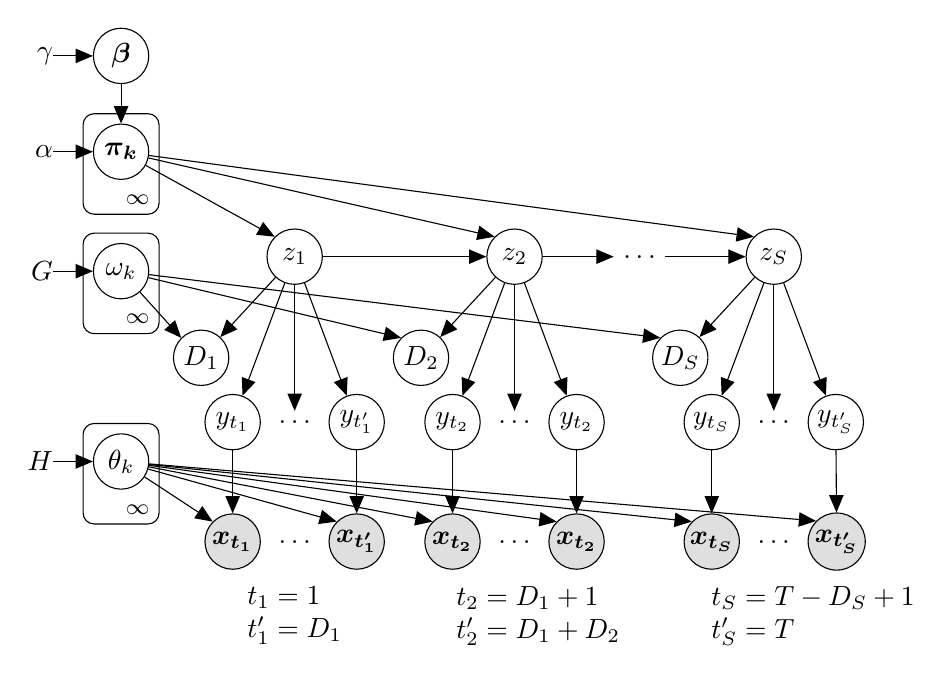
\begin{tikzpicture}[x=0.5cm,y=0.5cm]

  \node[obs] (x_t1){$\boldsymbol{x_{t_1}}$};
  \node[right=0.1 cm of x_t1] (x_dots1){$\ldots$};
  \node[obs, right=0.1 cm of x_dots1] (x_td1){$\boldsymbol{x_{t'_1}}$};

  \node[obs, right=of x_td1] (x_t2){$\boldsymbol{x_{t_2}}$};
  \node[right=0.1 cm of x_t2] (x_dots2){$\ldots$};
  \node[obs, right=0.1 cm of x_dots2] (x_td2){$\boldsymbol{x_{t_2}}$};

  \node[obs, right=1.0 cm of x_td2] (x_tS){$\boldsymbol{x_{t_{S}}}$};
  \node[right=0.1 cm of x_tS] (x_dotsS){$\ldots$};
  \node[obs, right=0.1 cm of x_dotsS] (x_tdS){$\boldsymbol{x_{t'_{S}}}$};

  %==================================================

  \node[latent, above=0.8 cm of x_t1] (y_t1){$y_{t_1}$};
  \node[right=0.1 cm of y_t1] (y_dots1){$\ldots$};
  \node[latent, right=0.1 cm of y_dots1] (y_td1){$y_{t'_1}$};

  \node[latent, right=of y_td1] (y_t2){$y_{t_2}$};
  \node[right=0.1 cm of y_t2] (y_dots2){$\ldots$};
  \node[latent, right=0.1 cm of y_dots2] (y_td2){$y_{t_2}$};

  \node[latent, right=1.0 cm of y_td2] (y_tS){$y_{t_{S}}$};
  \node[right=0.1 cm of y_tS] (y_dotsS){$\ldots$};
  \node[latent, right=0.1 cm of y_dotsS] (y_tdS){$y_{t'_{S}}$};

  %==================================================

  \node[latent, above=1.6 cm of y_dots1] (z_1){$z_1$};
  \node[latent, above=1.6cm of y_dots2] (z_2){$z_2$};
  \node[right=0.9 cm of z_2] (z_dots){$\ldots$};
  \node[latent, above=1.6cm of y_dotsS] (z_S){$z_S$};

  \node[latent, xshift=-0.4 cm, above= 0.1 cm of y_t1] (D_1){$D_1$};
  \node[latent, xshift=-0.4 cm, above= 0.1 cm of y_t2] (D_2){$D_2$};
  \node[latent, xshift=-0.4 cm, above= 0.1 cm of y_tS] (D_S){$D_S$};

  \node[latent, yshift=-0.5 cm, left=0.7cm of y_t1] (theta_k){$\theta_k$};
  \node[latent, above=1.7cm of theta_k] (omega_k){$\omega_k$};
  \node[latent, above=0.8 cm of omega_k] (pi_k){$\boldsymbol{\pi_k}$};

  \node[below=0.3cm of x_dots1, align=left] {$t_1 = 1$\\$t'_1 = D_1$};
  \node[xshift=0.3 cm, below=0.3cm of x_dots2, align=left] {$t_2 = D_1 + 1$\\$t'_2 = D_1 + D_2$};
  \node[xshift=0.5 cm, below=0.3cm of x_dotsS, align=left] {$t_S = T-D_S+1$\\$t'_S = T$};

  \node[const, left=of pi_k] (alpha){$\alpha$};
  \node[latent, above=of pi_k] (beta){$\boldsymbol{\beta}$};
  \node[const, left=of beta] (gamma){$\gamma$};
  \node[const, left=of omega_k] (lambda_q){$G$};
  \node[const, left=of theta_k] (lambda_theta){$H$};

  \edge{gamma}{beta};
  \edge{beta}{pi_k}
  \edge{alpha}{pi_k};
  \edge{lambda_q}{omega_k};
  \edge{lambda_theta}{theta_k};

  \edge{pi_k}{z_1.north west};
  \edge{pi_k}{z_2.north west};
  \edge{pi_k}{z_S.north west}

  \edge{z_1}{z_2};
  \edge{z_2}{z_dots};
  \edge{z_dots}{z_S}

  \edge{z_1}{D_1};
  \edge{z_1}{y_t1};
  \edge{z_1}{y_dots1};
  \edge{z_1}{y_td1};

  \edge{z_2}{D_2};
  \edge{z_2}{y_t2};
  \edge{z_2}{y_dots2};
  \edge{z_2}{y_td2};

  \edge{z_S}{D_S};
  \edge{z_S}{y_tS};
  \edge{z_S}{y_dotsS};
  \edge{z_S}{y_tdS};

  \edge{y_t1}{x_t1}
  \edge{y_td1}{x_td1}
  \edge{y_t2}{x_t2}
  \edge{y_td2}{x_td2}
  \edge{y_tS}{x_tS}
  \edge{y_tdS}{x_tdS}

  \edge{omega_k}{D_1.north west};
  \edge{omega_k}{D_2.north west};
  \edge{omega_k}{D_S.north west};

  \edge{theta_k}{x_t1.north west};
  \edge{theta_k}{x_td1.north west};
  \edge{theta_k}{x_t2.north west};
  \edge{theta_k}{x_td2.north west};
  \edge{theta_k}{x_tS.north west};
  \edge{theta_k}{x_tdS.north west};

  \plate{K_pi}{(pi_k)}{$\infty$};
  \plate{K_q}{(omega_k)}{$\infty$};
  \plate{K_theta}{(theta_k)}{$\infty$};

\end{tikzpicture}

\end{document}
